
\documentclass[a4paper,11pt]{article}
\usepackage{amsmath,amsthm,amsfonts,amssymb,amscd,amstext,vmargin,graphics,graphicx,tabularx,multicol} 
\usepackage[francais]{babel}
\usepackage[utf8]{inputenc}  
\usepackage[T1]{fontenc} 
\usepackage{pstricks-add,tikz,tkz-tab,variations}
\usepackage[autolanguage,np]{numprint} 

\setmarginsrb{1.5cm}{0.5cm}{1cm}{0.5cm}{0cm}{0cm}{0cm}{0cm} %Gauche, haut, droite, haut
\newcounter{numexo}
\newcommand{\exo}[1]{\stepcounter{numexo}\noindent{\bf Exercice~\thenumexo} : \marginpar{\hfill /#1}}
\reversemarginpar


\newcounter{enumtabi}
\newcounter{enumtaba}
\newcommand{\q}{\stepcounter{enumtabi} \theenumtabi.  }
\newcommand{\qa}{\stepcounter{enumtaba} (\alph{enumtaba}) }
\newcommand{\initq}{\setcounter{enumtabi}{0}}
\newcommand{\initqa}{\setcounter{enumtaba}{0}}

\newcommand{\be}{\begin{enumerate}}
\newcommand{\ee}{\end{enumerate}}
\newcommand{\bi}{\begin{itemize}}
\newcommand{\ei}{\end{itemize}}
\newcommand{\bp}{\begin{pspicture*}}
\newcommand{\ep}{\end{pspicture*}}
\newcommand{\bt}{\begin{tabular}}
\newcommand{\et}{\end{tabular}}
\renewcommand{\tabularxcolumn}[1]{>{\centering}m{#1}} %(colonne m{} centrée, au lieu de p par défault) 
\newcommand{\tnl}{\tabularnewline}

\newcommand{\bmul}[1]{\begin{multicols}{#1}}
\newcommand{\emul}{\end{multicols}}

\newcommand{\trait}{\noindent \rule{\linewidth}{0.2mm}}
\newcommand{\hs}[1]{\hspace{#1}}
\newcommand{\vs}[1]{\vspace{#1}}

\newcommand{\N}{\mathbb{N}}
\newcommand{\Z}{\mathbb{Z}}
\newcommand{\R}{\mathbb{R}}
\newcommand{\C}{\mathbb{C}}
\newcommand{\Dcal}{\mathcal{D}}
\newcommand{\Ccal}{\mathcal{C}}
\newcommand{\mc}{\mathcal}

\newcommand{\vect}[1]{\overrightarrow{#1}}
\newcommand{\ds}{\displaystyle}
\newcommand{\eq}{\quad \Leftrightarrow \quad}
\newcommand{\vecti}{\vec{\imath}}
\newcommand{\vectj}{\vec{\jmath}}
\newcommand{\Oij}{(O;\vec{\imath}, \vec{\jmath})}
\newcommand{\OIJ}{(O;I,J)}


\newcommand{\reponse}[1][1]{%
\multido{}{#1}{\makebox[\linewidth]{\rule[0pt]{0pt}{20pt}\dotfill}
}}

\newcommand{\titre}[5] 
% #1: titre #2: haut gauche #3: bas gauche #4: haut droite #5: bas droite
{
\noindent #2 \hfill #4 \\
#3 \hfill #5

\vspace{-1.6cm}

\begin{center}\rule{6cm}{0.5mm}\end{center}
\vspace{0.2cm}
\begin{center}{\large{\textbf{#1}}}\end{center}
\begin{center}\rule{6cm}{0.5mm}\end{center}
}



\begin{document}
\pagestyle{empty}
\titre{Contrôle 1}{Nom :}{Prénom :}{Classe}{Date}

\begin{flushleft}
\begin{tabular}{|m{9.5cm}|m{1.25cm}|m{1.25cm}|m{1.25cm}|m{1.25cm}|m{1.25cm}|}
\hline 
\textbf{Compétences} & \begin{center}
\textbf{N.E.}
\end{center} & \begin{center}
\textbf{M.I.}
\end{center} & \begin{center}
\textbf{M.F.}
\end{center}  & \begin{center}
\textbf{M.S.}
\end{center} & \begin{center}
\textbf{T.B.M.}
\end{center} \\ 
\hline 
Je dois savoir traduire en langage mathématique une situation réelle &  &  & & &\\
\hline 
Je dois savoir démontrer : utiliser un raisonnement logique et des règles établies (propriétés, théorèmes, formules) pour parvenir à une conclusion&  &  & & &\\
\hline


\end{tabular} 
\end{flushleft}

\textit{N.E = Non évalué ; M.I. = Maîtrise insuffisante ; M.F. = Maîtrise fragile ; M.S. = Maîtrise satisfaisante ; T.B.M. = Très bonne maîtrise}\\

\vspace*{0.3cm}
\exo{2} Calculer les expressions suivantes \textbf{en détaillant toutes les étapes de calculs.}

\bmul{2}

$D= (-5) + 10 - (-23) + (-55) - (+100)$\\



\columnbreak

$U= (-2,05) - (-6,1)+5,9 -10,8+2,05-(-9,5)$\\

\emul

\exo{2} Donner le signe des calculs suivant en justifiant votre réponse. 

\bmul{2}

$F= (-5) \times (-1,7) \times (+3) \times (-8) \times (+6,4) \times 9$\\

\columnbreak

$D=-\dfrac{-12 \times 4,5 \times (-1) \times (-3,1)}{3 \times (-10,02) \times 7}$


\emul




\vspace*{0.3cm}


\exo{5} Lors d'un concours d'entrée dans une école, les étudiants doivent répondre à un QCM de 30 questions.

\bmul{2}
\setlength{\fboxrule}{1pt}
\begin{flushleft}
\framebox{\begin{minipage}{\linewidth}

\vspace*{0.2cm}


\textbf{Doc 1} \\

Le barème est le suivant : 
\bi
\item 3 points par bonne réponse ;
\item -1,5 points par mauvaise réponse ;
\item 0 point par absence de réponse.
\ei

\vspace*{0.2cm}
\end{minipage}}
\end{flushleft}

\columnbreak

\setlength{\fboxrule}{1pt}
\begin{flushleft}
\framebox{\begin{minipage}{\linewidth}

\vspace*{0.2cm}


\textbf{Doc 2} \\

\bi
\item Mia a répondu à toutes les questions et 20 de ses réponses sont justes.
\item Jules a répondu à 23 questions et 6 de ses réponses sont fausses.
\item Amy a répondu à seulement 16 questions et ses réponses sont toutes justes.
\ei


\vspace*{0.2cm}
\end{minipage}}
\end{flushleft}


\emul

\q \initqa \qa Quel est le nombre maximum de points que l'on peut obtenir à ce QCM? Justifier votre réponse.\\
\qa Quel est le nombre minimum de points que l'on peut obtenir à ce QCM? Justifier votre réponse.\\

\q \initqa \qa Écrire une expression qui permet de calculer  le nombre de points obtenus par Mia. Donner le résultat de ce calcul.\\
\qa Qui de Mia, Jules et Amy a obtenu le plus de points ? Justifier votre réponse.\\

\q Milo a obtenu 60 points. Proposer un nombre de questions auxquelles il aurait répondu ainsi que le nombre de réponses justes.\\

\vspace*{0.3cm}

\newpage

\exo{5} 
\bmul{2}
Une échelle appuyée contre un mur vertical se trouve à 5 m du mur. (la figure n'est pas à l'échelle) Elle glisse le long du mur de 80 cm.\\
 Elle se trouve à 11,2 m du sol et s'est éloignée d'une longueur de $x$ en m sur le sol.\\
 
$\rightarrow$ \textbf{Calculer la longueur $x$.}\\

\textit{Toute trace de recherche, même incomplète, ou d'initiative même infructueuse, sera prise en compte dans l'évaluation.}\\

\columnbreak

\includegraphics[scale=1.4]{exothm1.eps} \\

\emul


\vspace*{0.5cm}

\exo{6} Un professeur de SVT demande aux élèves d'une classe de sixième de faire germer des graines de blé chez eux.\\

Le professeur donne un protocole expérimental à suivre.
\bi
\item Mettre en culture sur du coton dans une boîte placée dans une pièce éclairée, de température entre \\
20 \degre C et 25\degre C.
\item Arroser une fois par jour.
\item Il est possible de couvrir les graines avec un film transparent pour éviter l'évaporation de l'eau.\\
\ei

Le tableau ci-dessous donne les tailles des plantules (petites plantes) des élèves à 10 jours après la mise en germination.\\


\renewcommand{\arraystretch}{1.8}

\begin{tabular}{|c|c|c|c|c|c|c|c|c|c|c|c|}
\hline 
Taille (en cm) & 0 & 8 & 12 & 14 & 16 & 17 & 18 & 19 & 20 & 21 & 22 \\ 
\hline 
Effectifs & 1 & 2 & 2 & 4 & 2 & 2 & 3 & 3 & 4 & 4 & 2 \\ 
\hline 
\end{tabular} 

\vspace*{0.4cm}

\initq \q  Combien de plantules ont une taille qui mesure au plus 12 cm ?\\

\q Donner les valeurs extrêmes de cette série.\\

\q Quel est effectif total de cette série ?\\

\q Quel pourcentage des élèves de la classe a obtenu une plantule qui mesure au plus 18 cm ?\\


\q On considère qu'un élève a bien respecté le protocole si la taille de la plantule à 10 jours est supérieure ou égale à 14 cm.\\
Quel pourcentage des élèves de la classe a bien respecté le protocole ?\\



\exo{} BONUS \\
Une corde non élastique de 6 mètres est attachée au sol entre deux piquets distants de 5 mètres. \\
Tom tire la corde en son milieu et la lève aussi haut que possible.\\

Données numériques : Tom mesure 1 m 68.\\

Peut-il passer en dessous sans se baisser ? Justifier votre réponse.\\


\end{document}
